\section{Detailed study of Equipments}

%\begin{figure}
%  \centering
%  \includegraphics[width=4in]{gecko}
%  \caption[Close up of \species{Hemidactylus}]
%  {Close up of \species{Hemidactylus}, which is part the genus of the gecko family. It is the second most 
%    speciose genus in the family.}
%\end{figure}

%\newtheorem{name}{Printed output}



\subsection{Tank}



large grey plastic vessel

Should we line the inner surface? Stan has been investigating various
non-reflective surfaces

needs investigation into water compatibility and possible emanation





\subsection{Mechanical Gantry System}


As noted before in the introduction, the PTF measurements are made by moving a pair of optical heads to
different positions to illuminate the 20\" PMT.  This motion is accomplished by having the optical heads be on
a pair of moveable gantries.  The gantries provide movement in five different axes: X, Y, Z, rotation and tilt.
The X, Y and Z motion is on three separate linear stages driven by stepper motors,
with the dimensions of the stages being XXXYYY, XXXYYY
and XXXYYY.  The tilt motion is provided by a rotary stage; the tilt motion of the optical head is
provided by a XXXYYY driven by a stepper motor.
This is all shown diagramatically in Figure XXXYYY; these elements are all duplicated for
the two gantries.  The gantry motors are controlled by a Galil 8143 motor controller; the controller is configured
over an ethernet link.  The configuration is handled in a MIDAS program and webpage, described in Section
\ref{Sec:DAQ_Controls}.

Limit switches provide some degree of protection against collisions.  But the two gantries can
be moved into the same space; so additional higher-level collision avoidance has been
programmed into the software control programs.



Various tests have been performed to understand the reproducibility of the gantry motion.  These tests have shown
XXXYYY






\subsection{Optical System/Head}

Shimpei

collimate/polarize the incoming light

watertight

how to manipulate?

new sources?


\subsubsection{Phidget Accelerometer and Magnetometer}
\label{Sec:PhidgetAccMag}.

The optiocal heads also contain small electronic cards with 3-axis accelerometers and
magnetometers.  These cards are Phidget 1044 boards, which are readout by USB \cite{PhidgetRef}.
We use the accelerometer to measure the tilt of the optical head; the tilt drive system
otherwise has no other system for measuring the tilt.

The magnetometer is used to measure the magnetic field near the 20\" PMT.  We use the Phidget
readings to ensure that we are correctly cancelling the ambient magnetic field, as described
in more detail in Section \ref{Sec:MagFieldCompensation}.
One problem with the Phidgets is that magnetometers are not designed for high precision or accuracy  measurements.
We therefore find that, even after the calibration procedure specified by Phidget, that the
magnetic field measurements only have an accuracy of XXXYYY mG.


\subsection{Optical Fibre}
ideal wavelength range is 350--650~nm

consider bending radius

throughput

tested three samples

selected FT200UMT

good transmission across the wavelengths tested~(378--777~nm)

seemed almost unaffected by curvature

fibre must reach several metres from laser through manipulator to the
optical head

how to mount, etc. to prevent tangles, excessive bending, etc.


\subsection{Magnetic Field Compensation}
\label{Sec:MagFieldCompensation}

The PMTs are sensitive to magnetic field conditions in its electron-path trajectory. For studies of the PMT response to be possible, the magnetic field in the PTF must be well-understood and controlled.

The PTF is located a few hundred meters away from TRIUMF's cyclotron, which produces a magnetic field of around 1800 mG in magnitude in the PTF when turned on. Even when the cyclotron is turned off, surrounding structural material in the building can be magnetized and affect the magnetic fields in the PTF. 

The magnetic field compensation set-up in the PTF involves passive compensation using GIRON sheets as magnetic shielding, as well as active compensation using three pairs of square coils, modelled after Helmholtz coils. Thorough magnetic field compensation procedures have been developed for both when TRIUMF's cyclotron is on and off, and the magnetic field is constantly being monitored by the Phidgets, devices that act as both magnetometers and accelerometers (see \ref{Sec:PhidgetAccMag} for more about the Phidgets). 

\subsubsection{Passive Compensation - GIRON Magnetic Shielding}

The magnetic fields in the PTF exhibit large gradients in each direction. The GIRON magnetic shielding helps reduce these gradients to make the magnetic field in the PMT volume more uniform. This is especially important for the z-component of the magnetic field, as the cyclotron at TRIUMF produces large magnetic fields in the z-direction. The magnitude of this magnetic field changes with the distance from the cyclotron, thereby creating a gradient.

The GIRON sheets were purchased from Less EMF. Figures~\ref{fig:bfield_gironeffects_a} and \ref{fig:bfield_gironeffects_b} show how the gradient observed in the z-component of the magnetic field in the PTF is reduced by $ 63\pm3 $\% by adding one layer of GIRON flooring (see \ref{Appendix:MagneticFieldGradientCalculations} for calculations).
Figure~\ref{fig:bfield_gironeffects_c} shows that adding a second layer of GIRON flooring does not reduce the gradient in the magnetic field. The main reason for keeping the second layer of GIRON flooring is to ensure that there are no gaps between the GIRON sheets.
%
\begin{figure}[htbp]
  \begin{center}
    \subfloat[No GIRON flooring\label{fig:bfield_gironeffects_a}]{
      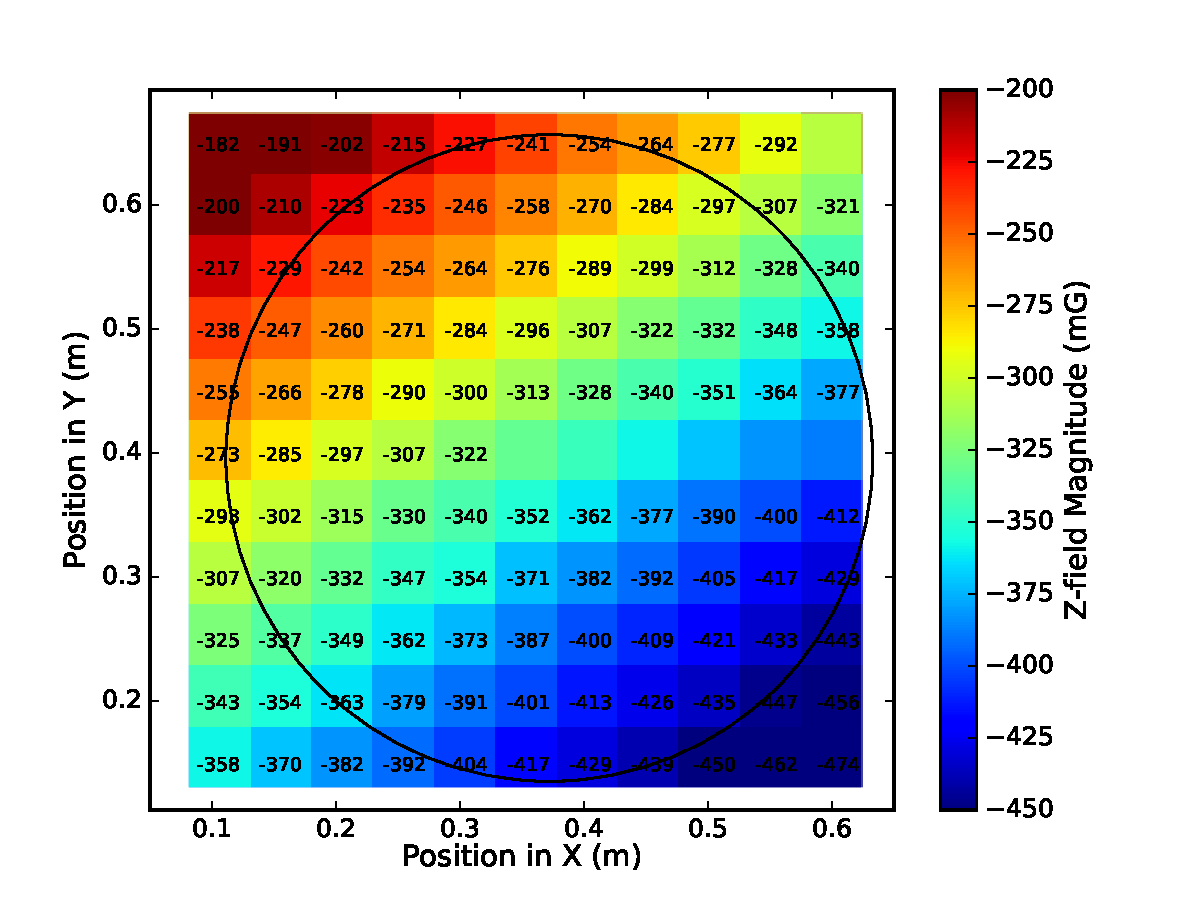
\includegraphics[width=0.5\textwidth]{bfield_0_no_compensation_z_clrbaredit.pdf}
    }\\
    \vspace{-3 mm}
    \subfloat[One layer of GIRON flooring\label{fig:bfield_gironeffects_b}]{
      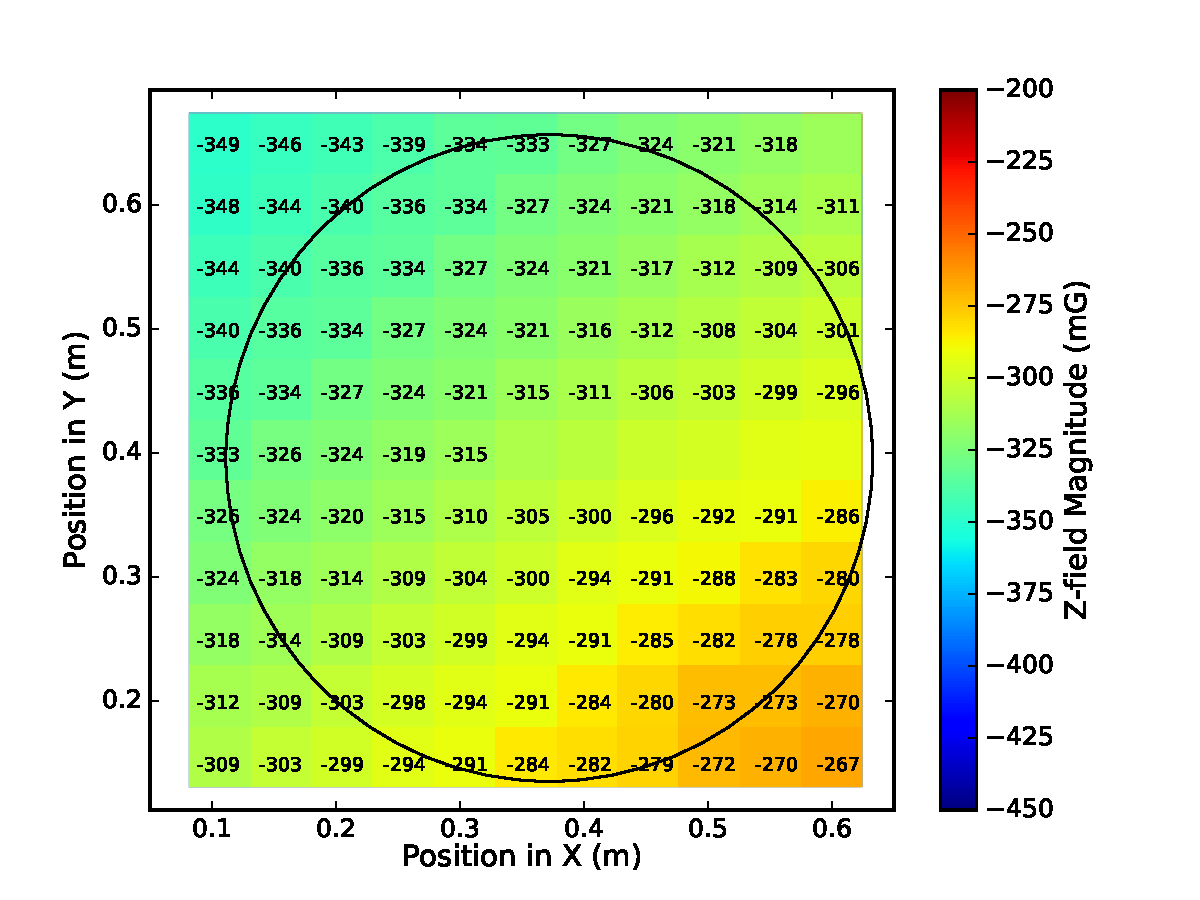
\includegraphics[width=0.5\textwidth]{bfield_1_1layerGIRON_coilsOff_z_clrbaredit.pdf}
    }\\
    \vspace{-3 mm}
    \subfloat[Two layers of GIRON flooring\label{fig:bfield_gironeffects_c}]{
      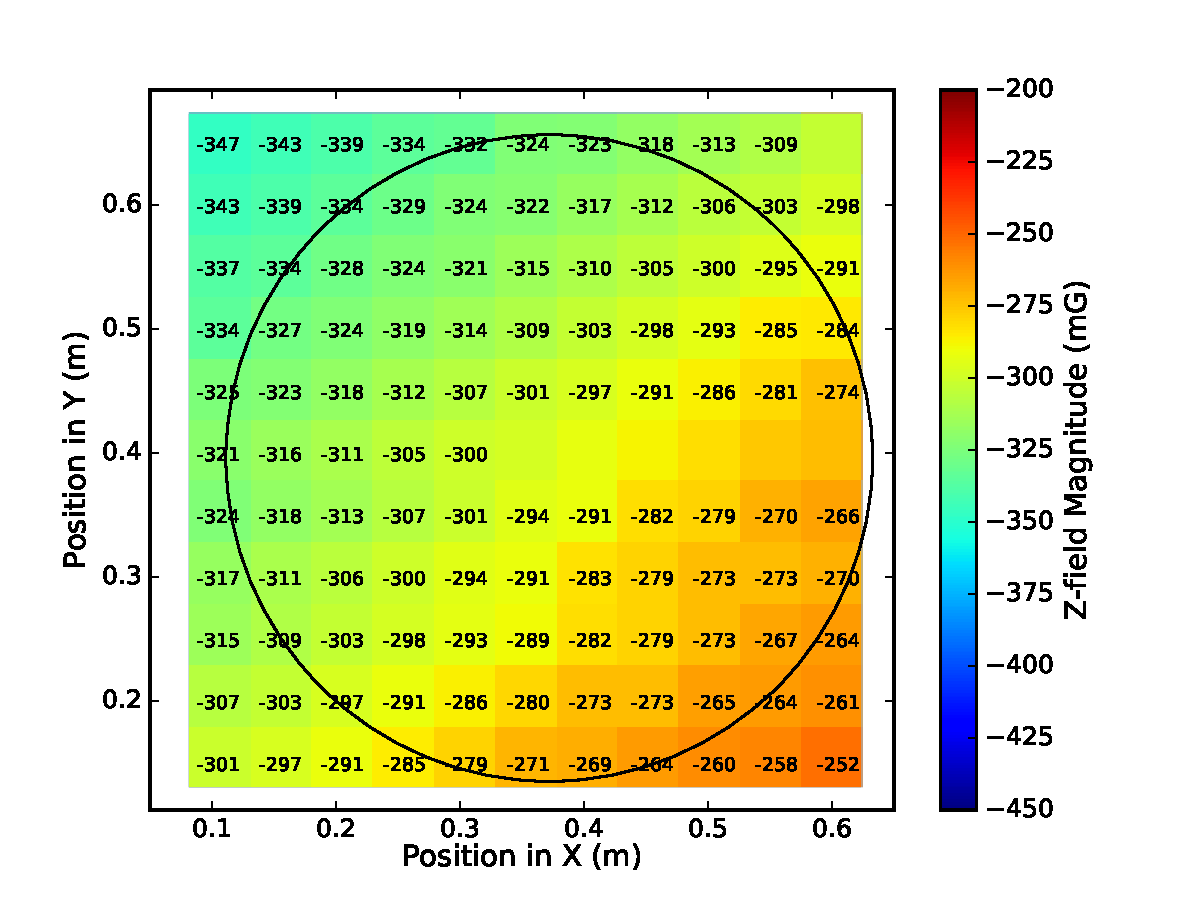
\includegraphics[width=0.5\textwidth]{bfield_2_2layerGIRON_coilsOff_z_clrbaredit.pdf}
    }
  \caption{Plots of the z-component of the magnetic field in the x-y plane containing the center of the PMT volume, with: no GIRON flooring (\ref{fig:bfield_gironeffects_a}), one layer of GIRON flooring (\ref{fig:bfield_gironeffects_b}), and two layers of GIRON flooring (\ref{fig:bfield_gironeffects_c}). The circle outlines the position of the 20\" PMT when it is being measured in the PTF. The GIRON flooring helps reduce the magnetic field gradient along the x-y plane.}
  \label{fig:bfield_gironeffects}
  \end{center}
\end{figure}
%

As shown in Figure~\ref{fig:bfield_gironeffects}, the GIRON flooring helps reduce the magnetic field gradients in the x-y plane. Similarly, GIRON sheets have been wrapped around the PTF tank into a cylindrical shape, as shown in Figure~\ref{fig:coils} to help reduce the magnetic field gradients in the z-direction. Figure~\ref{fig:bfield_gironcylinder} shows how the gradient of the x-component of the magnetic field is reduced from $ 75\pm18 $mG/m to almost no gradient in the z-direction with the cylinder in place.
%
\begin{figure}[htbp]
  \begin{center}
    \subfloat[Without GIRON cylinder around tank\label{fig:bfield_gironcylinder_a}]{
      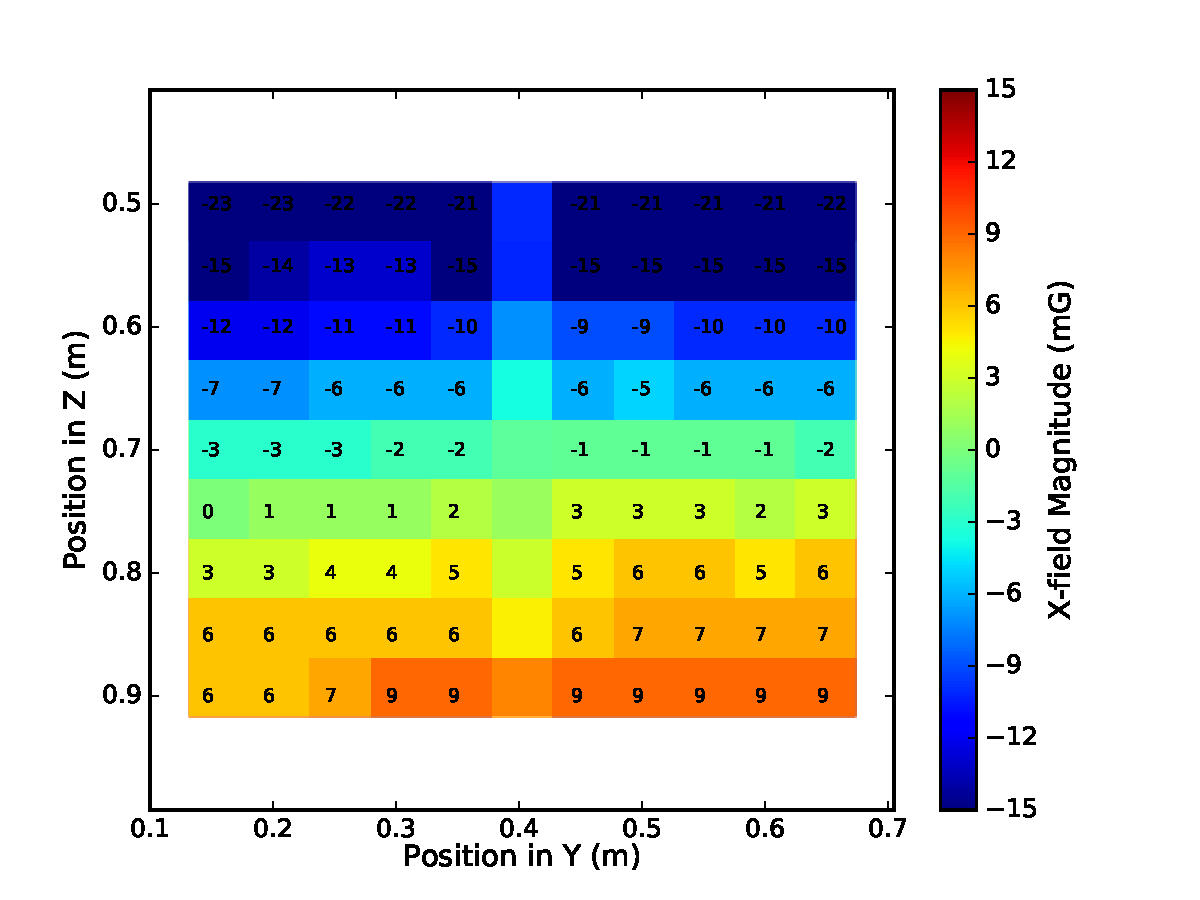
\includegraphics[width=0.5\textwidth]{bfield_3_2layerGIRON_coilsOn_x352_x.pdf}
    }\\
    \vspace{-3 mm}
    \subfloat[With GIRON cylinder around tank\label{fig:bfield_gironcylinder_b}]{
      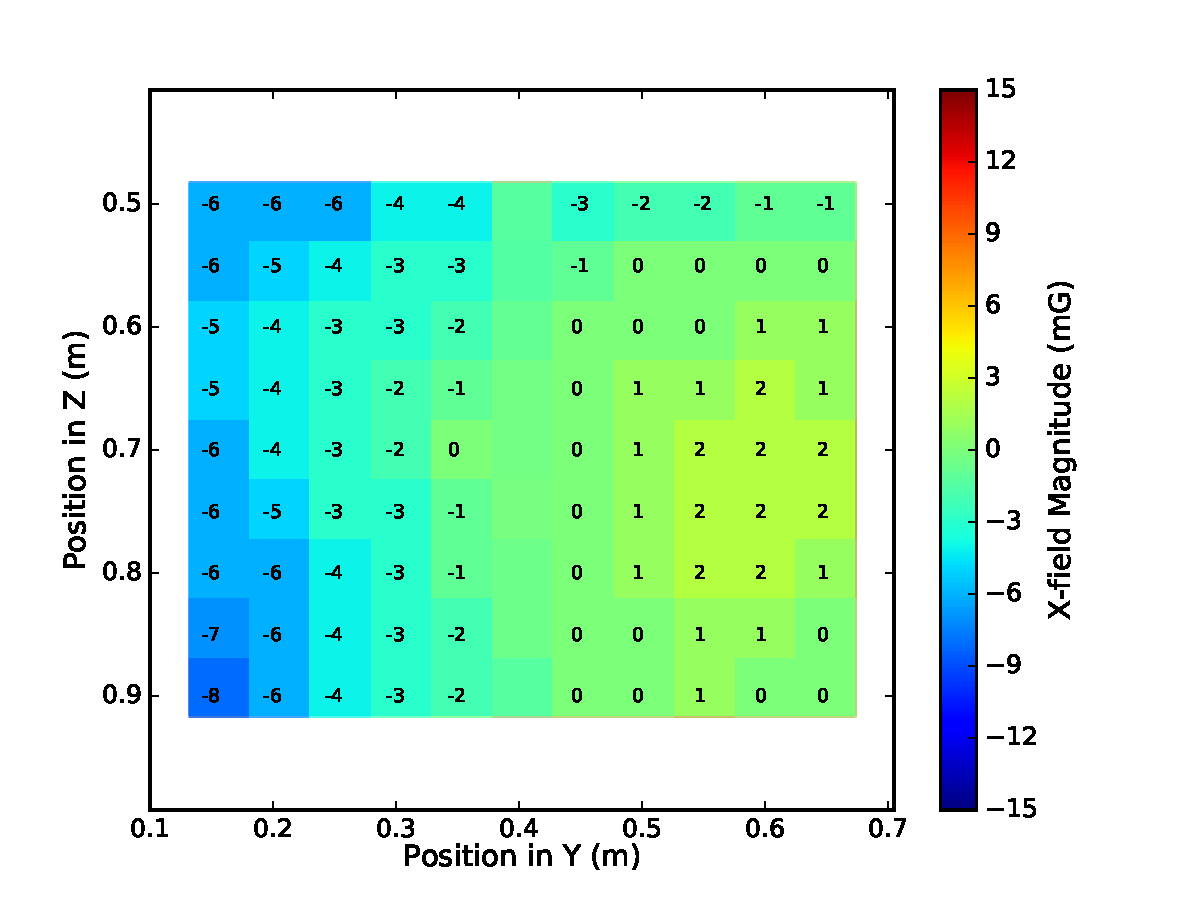
\includegraphics[width=0.5\textwidth]{bfield_4_FullCompensation_x352_x.pdf}
    }
  \caption{Plots of the x-component of the magnetic field in the y-z plane containing the center of the PMT volume, without the cylindrical GIRON shielding (\ref{fig:bfield_gironcylinder_a}), and with the cylindrical GIRON shielding around the PTF tank (\ref{fig:bfield_gironcylinder_b}). In both cases, there are two layers of GIRON flooring and the compensation coils are tuned to obtain a field of 0 mG at the center of the scan region. The GIRON cylinder helps reduce the magnetic field gradient in the z-direction.}
  \label{fig:bfield_gironcylinder}
  \end{center}
\end{figure}
%

\subsubsection{Active Compensation - Helmholtz Coils}

While passive compensation helps reduce the gradient in the magnetic field, active compensation with Helmholtz-like coils help reduce the magnitude of the magnetic field.

The six coils used are wrapped around square frames made of wood (see Figure~\ref{fig:coils}). Coils 1 and 2 are used to control the z-component of the magnetic field, coils 3 and 4 the x-component, and coils 5 and 6 the y-component.

Detailed coil specifications are given in table~\ref{tab:coil_specs}.
%
\begin{figure}[h]
  \begin{center}
  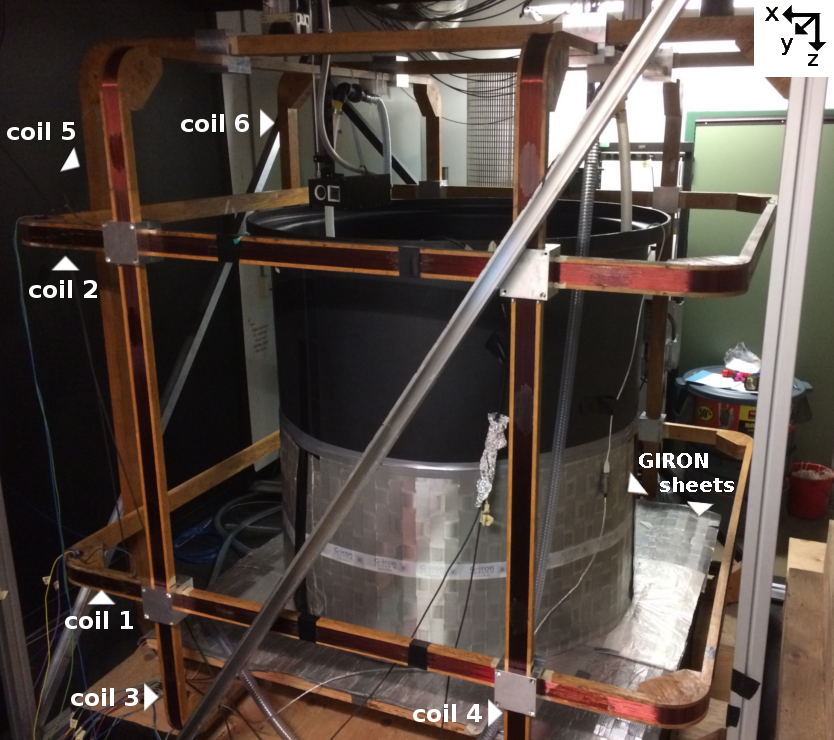
\includegraphics[width=0.6\textwidth]{bfield_PTFcoilconfig.png}
  \caption{Square coils are used for active compensation of the magnetic field.}
  \label{fig:coils}
  \end{center}
\end{figure}
%
\begin{table}[h]
\begin{center}
  \begin{tabular}{|c|c c c c|}
    \hline
    Coil number & Side length (cm) & Wire (AWG) & Number of turns & Resistance ($\Omega$)\\
    \hline\hline
    1 & 189 & 14 & 52 & 3.8 \\
    2 & 189 & 14 & 52 & 3.8 \\
    3 & 196 & 14 & 52 & 3.8 \\
    4 & 196 & 14 & 52 & 3.9 \\
    5 & 204 & 12 & 260 & 11.1 \\
    6 & 204 & 12 & 260 & 11.1 \\
    \hline
  \end{tabular}
\end{center}
\caption{Compensation coil specifications}
\label{tab:coil_specs}
\end{table}
%

The coils are surrounded by aluminum framing that is a part of the gantry system's structural support. The position of the coils are fixed with respect to this aluminum framing, and with one another (see \ref{Appendix:CoilPositions} for a diagram of the precise coil positions).

Although the geometry of these coil pairs are not exactly that of Helmholtz coils (the coils are square instead of circular, and the distance between the coils are adjusted to accomodate for the movement of the gantries), the set-up has been thoroughly studied to find the optimum voltage combinations for controlling magnetic fields.

\subsubsection{Magnetic Field Studies}

The use of GIRON magnetic shielding makes it more challenging to quantify the current-to-magnetic-field relations in the PTF. Likewise, calibration of the compensation coils was accomplished through detailed experimentation.

The magnetic fields are mapped at 5-cm intervals in a volume of 0.5 m by 0.5 m by 0.4 m. The scan volume is centered about the center of the 20\" PMT's electron-path trajectory, where the PMT's cross-sectional diameter is largest. By ensuring that the scan volume includes the entire volume of the 20\" PMT, the magnetic field at every point inside the PMT can be interpollated from the measurements.

Figures~\ref{fig:bfield_gironeffects} and \ref{fig:bfield_gironcylinder} are examples of the plots produced through these mangetic field scans. \ref{Appendix:MagneticFieldScanPlots} contains a few more plots for reference.

The tuning of the coil currents was accomplished by placing one of the Phidgets at the center of the scan volume and adjusting the currents so that the Phidget measures a magnetic field value of 0 mG. The Phidget is then moved around the scan volume to map the magnetic field and ensure that the fields would be uniform throughout the PMT volume.

The magnetic field studies show that the final magnetic-filed-compensation set-up, with GIRON flooring and a cylindrical GIRON shield around the tank coupled with compensation coils, is ideal for producing uniform magnetic fields within the PMT volume for both when the cyclotron is turned on and off. The coil current settings for full compensation have been recorded, and repeatability has also been tested to show that the magnetic fields in the entire scan volume can be reproduced to within $\pm7$ mG.


\subsubsection{Degaussing}

GIRON exhibits magnetic hysteresis: once GIRON is magnetized, simply applying a magnetic field in the opposite direction is not enough to demagnetize GIRON, as some of the magnetic dipoles in the GIRON remain. Therefore a systematic degaussing procedure was developed to demagnetize the GIRON shielding using the compensation coils.

Degaussing involves removing the non-random magnetic dipoles in the GIRON shielding by exposing it to external magnetic fields that are alternating in direction. The magnitude of this alternating field is gradually reduced so that the PMT volume eventually reaches a state in which the magnetic fields are of zero magnitude.

The systematic degaussing procedure has proven to be a reliable method that guarantees reproducible magnetic field conditions. 

%***NOTES***

%assess magnetic shielding, magnetic compensation

%GIRON magnetic shielding (http://www.lessemf.com/)

%GIRON frame

%Helmholtz coils, could include the dimensions, wire details, measured resistance

%could describe the testing we have done, eg. setting the voltage and measuring the field with a handheld gaussmeter

%Phidget on each gantry

%coil positioning, maybe outside frame supports for coils, precision measurement of coil position

%direction of current and maximum external fields

%consider when synchrotron is on

%control development

%might have to do each scan more than once (debugging, etc.)

%Magnetic field scans:
%\begin{itemize}
%\item{\bf Scan 0} no current, no GIRON, calculate the the fields that are needed from the coils
%\item{\bf Scan 1} set currents
%\item{\bf Scan 2} one layer of GIRON
%\item{\bf Scan 3} two layers of GIRON
%\end{itemize}


\subsection{Light Tightness/Dark room}

The gantry system is surrounded by a double set of heavy black
curtains on a overhead rail.  The black curtains provided light tightness.
As an additional darkening step, the lights in the rest of the PTF room
are turned off whenever the 20\" PMT is powered on.


\subsection{Water System}
Andy and Peter

Water circulation and filtration system

degassification is a major item


\subsection{DAQ/Controls}
\label{Sec:DAQ_Controls}

The PTF DAQ uses the MIDAS framework \cite{MIDASRef}.  The main goals of the PTF DAQ are

\begin{enumerate}
\item Control of the gantry motors and scan sequencing
\item Digitization of the 20\" PMT and monitor PMT signals 
\item Environmental monitoring
\end{enumerate}

We will describe in more detail each of these points in turn in the following sections.

\subsubsection{Motor Control and Scan Sequencing}


\subsubsection{PMT Signal Digitization}

To digitize the signals from the 20\", monitor and receiver PMTs we use a fast waveform digitizer; specifically
we use the 500 megasample per second V1730 Module from Caen \cite{V1730Ref}.  The fast, high precision digitization rate ensures that we
are able to accurately measure the time and charge for single photoelectron pulses from all the PMTs.


\subsubsection{Environmental Monitoring}




collision avoidance is in place and working

collision avoidance in the xz-plane will be necessary once a PMT is in place

further testing and refinement will take about 1 week

how to mount PMTs in the tank




\subsection{Photosensor}

measure different PMTs
\begin{itemize}
\item SK 20 inch
\item IceCube 13 inch, contact Darren Grant
\item hybrid photosensor
\end{itemize}

should contact Japanese, how many PMTs and when?

LBNE has made measurements

angular dependence

magnetic field dependence


measurements before the tank is filled with water

HV and signal must reach from high voltage power supply to the optical
head

